% Бүлэг 1

\pagecolor{ChapterYellow}
\chapter{\ttitle\spaceсудалгааны хэсэг} % Бүлгийн нэр
\label{Chapter1} % Энэ бүлэг рүү ишлэл хийх бол \ref{Chapter1} командыг ашигла 

%-------------------------------------------------------------------------------

% Агуулгад ашигласан хэвшүүлэлтийн зарим командын тодорхойлолт
\newcommand{\keyword}[1]{\textbf{#1}}
\newcommand{\tabhead}[1]{\textbf{#1}}
\newcommand{\code}[1]{\texttt{#1}}
\newcommand{\file}[1]{\texttt{\bfseries#1}}
\newcommand{\option}[1]{\texttt{\itshape#1}}

%-------------------------------------------------------------------------------

%---------------------------------------------------------------------------------------
%	SECTION 1
%---------------------------------------------------------------------------------------
\pagecolor{white}
\section{\ttitle\spaceтухай танилцуулга}

Энэхүү төсөл нь дугуйтай хүмүүст өөрийн явж буй чиглэлд ойр байгаа хүргэлтүүдийг хийх боломж олгох бөгөөд, дугуйтай хүмүүс машинаас илүү хурдан явах боломжтой. Хүргэгчийн байршлыг хэрэглэгчид байнга мэдээлэнэ мөн хүргэгчид үнэлгээ өгөх боломжтой учир найдвартай.

Системийг ашиглахын тулд хэрэглэгч интернет сүлжээнд холбогдсон байх ба системд бүртгэлтэй байх ёстой бөгөөд бүртгэлээ сошиал хаягаараа нээх аль эсвэл бүртгүүлэх форумыг бөглөж бүртгүүлнэ. Үйлчлүүлэгч нь системээр дамжуулж хүргэлт захиалах, үйлчилгээ бүрд үнэлгээ өгөх, хувийн мэдээллээ шинэчлэх зэрэг үйлдлүүдийг гүйцэтгэнэ. Харин хүргэгчийн хувьд үйлчлүүлэгчийн захиалгаар үйлчилгээг үзүүлэх зэрэг үйлдлүүдийг гүйцэтгэнэ.

%---------------------------------------------------------------------------------------
%	SECTION 2
%---------------------------------------------------------------------------------------
\section{Ижил төстэй системийн судалгаа}

\subsection{Courier апп}
. Уг апп-ны давуу талуудыг доор дурдвал.
\begin{enumerate}[noitemsep]
	\item Байнга хүргэлт хийдэг газруудаа хадгалах боломжтой.
	\item Хэрэглэхэд тун энгийн.
	\item Олон хэлний сонголттой.
	\item Төлбөрийн картны мэдээллийг хадгалах боломжтой.
    \item Мобайл апп-аас гадна вэб апптай.
\end{enumerate}

\noindent Сул талууд:
\begin{enumerate}[noitemsep]
	\item Хэрэглэгчийн интерфэйс муутай.
	\item Зарим утасны хувилбар дээр ажиллах боломжгүй.
	\item Хүргэлтийн мэдээллээ шалгахын тулд заавал код авна.
\end{enumerate}

Зураг~\ref{fig:courier}--т Courier аппликэйшны дэлгэцүүдийг жишээ болгон харуулав.

\begin{figure}[H]
	\centering
    \subcaptionbox{Хүргэлт шинээр үүсгэх}{
        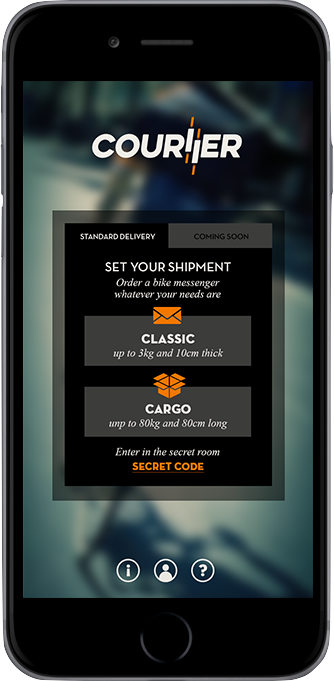
\includegraphics[width=.3\textwidth, frame]{Figures/ijil/courier1.png}
    }
    \hfill
    \subcaptionbox{Хүргэлтийн очих байршил сонгох}{
        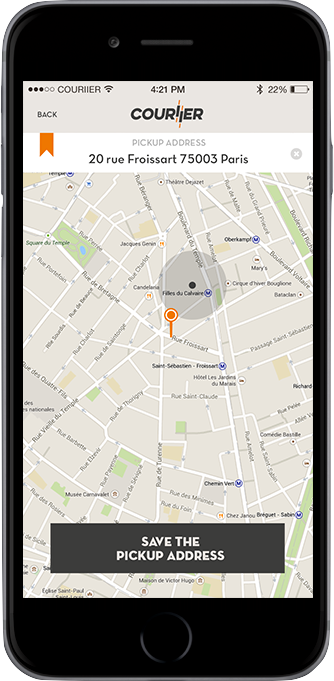
\includegraphics[width=.3\textwidth, frame]{Figures/ijil/courier2.png}
    }
    \hfill
    \subcaptionbox{Хүргэлтийн мэдээллүүд оруулах}{
        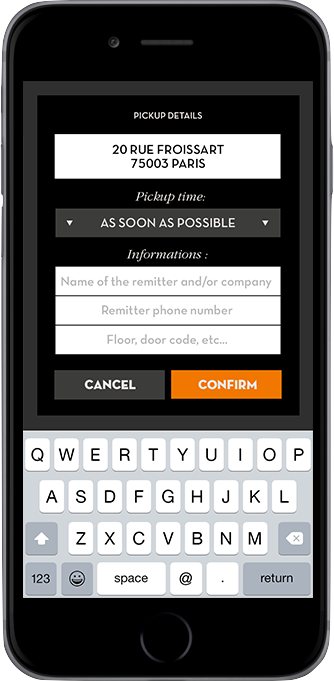
\includegraphics[width=.3\textwidth, frame]{Figures/ijil/courier3.png}
    }
	\caption{Courier аппликэйшны дэлгэцийн интерфэйс}
	\label{fig:courier}
\end{figure}


\subsection{DBike Messenger апп}
Уг аппын давуу талуудыг доор дурдвал.
\begin{enumerate}[noitemsep]
    \item Хүргэгч болон хэрэглэгч 2 хоорондоо чатлах боломжтой.
    \item Түүх харах боломжтой.
    \item Төлбөрийн системийг системд багтаасан.
    \item Мобайл апп-аас гадна вэб апптай.
\end{enumerate}

\noindent Сул талууд:
\begin{enumerate}[noitemsep]
    \item Үнийг хэрэглэгч биш систем тогтооно.
	\item Хэрэглэгчийн интерфэйс муутай.
	\item Хэтэрхий олон нэмэлттэй, хэрэглэхэд төвөгтэй.
	\item Зарим утасны хувилбар дээр ажиллах боломжгүй.
	\item Утас амархан ачаалладаг.
\end{enumerate}


Зураг~\ref{fig:dbike}--т DBike Messenger аппликэйшны дэлгэцүүдийг жишээ болгон харуулав.
\begin{figure}[H]
	\centering
    \subcaptionbox{Хүргэлтүүдийн жагсаалт}{
        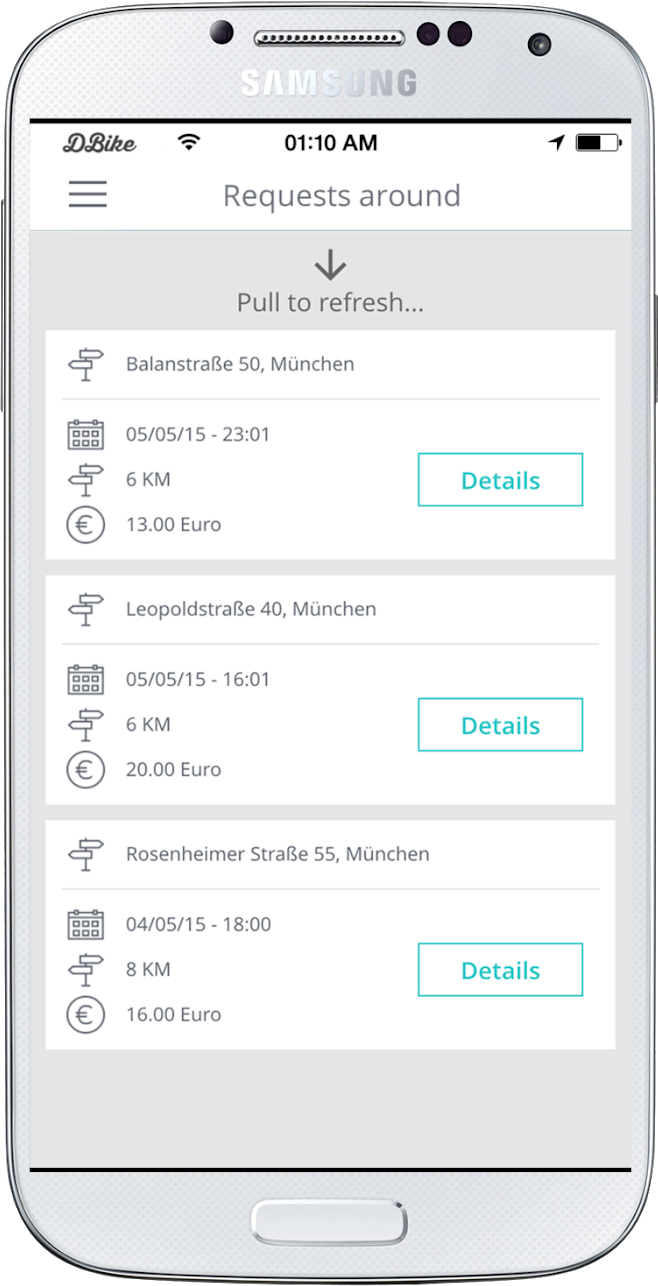
\includegraphics[width=.3\textwidth, frame]{Figures/ijil/dbike1.png}
    }
    \hfill
    \subcaptionbox{Хүргэлтийн дэлгэрэнгүй}{
        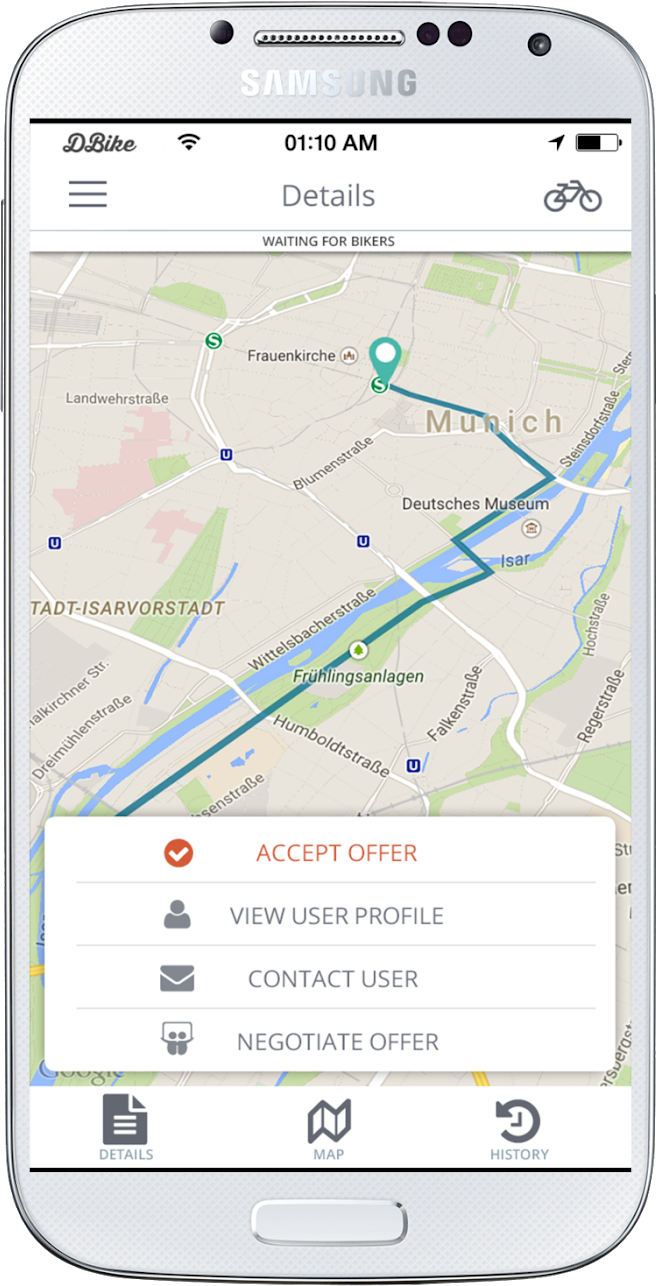
\includegraphics[width=.3\textwidth, frame]{Figures/ijil/dbike2.png}
    }
    \hfill
    \subcaptionbox{Хүргэлтийн төлөв өөрчлөх}{
        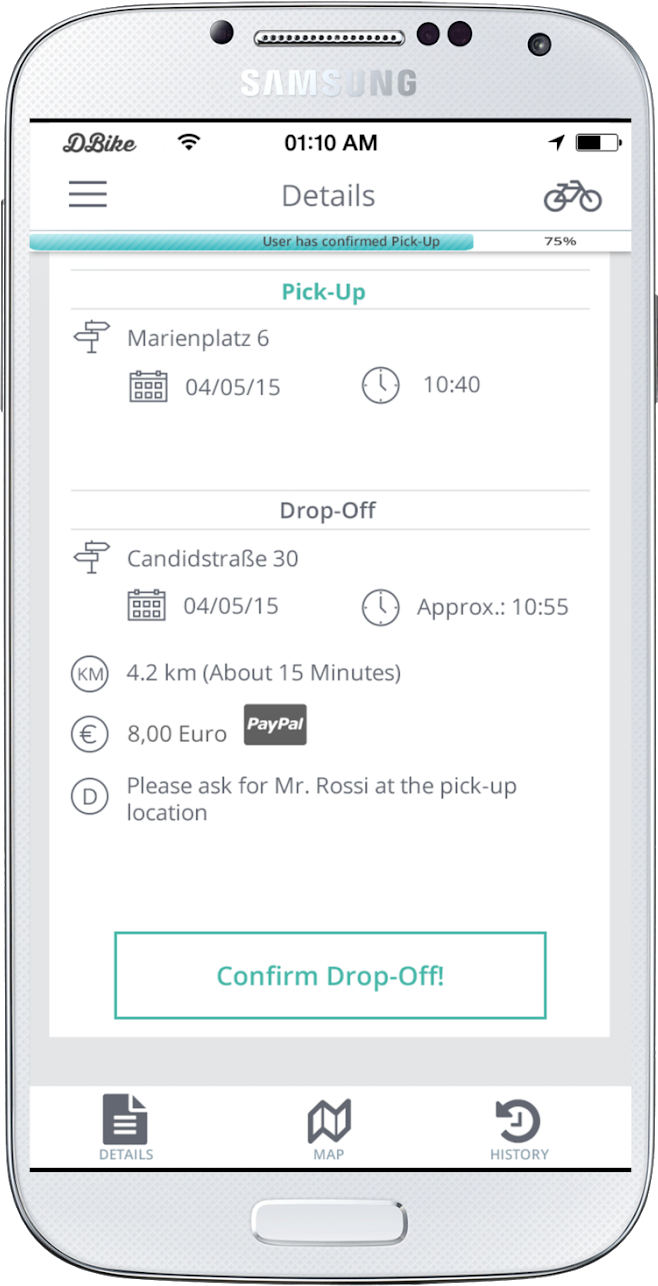
\includegraphics[width=.3\textwidth, frame]{Figures/ijil/dbike3.png}
    }
	\caption{DBike Messenger аппликэйшны дэлгэцийн интерфэйс}
	\label{fig:dbike}
\end{figure}



%---------------------------------------------------------------------------------------
%	SECTION 3
%---------------------------------------------------------------------------------------
\section{Тоон судалгаа баримт}

Зураг~\ref{fig:employee}--т АНУ-д үйл ажиллагаа явуулдаг хүргэлтийн байгууллагуудын ажилчдын тоон өсөлтийг харуулав.
\begin{figure}[H]
	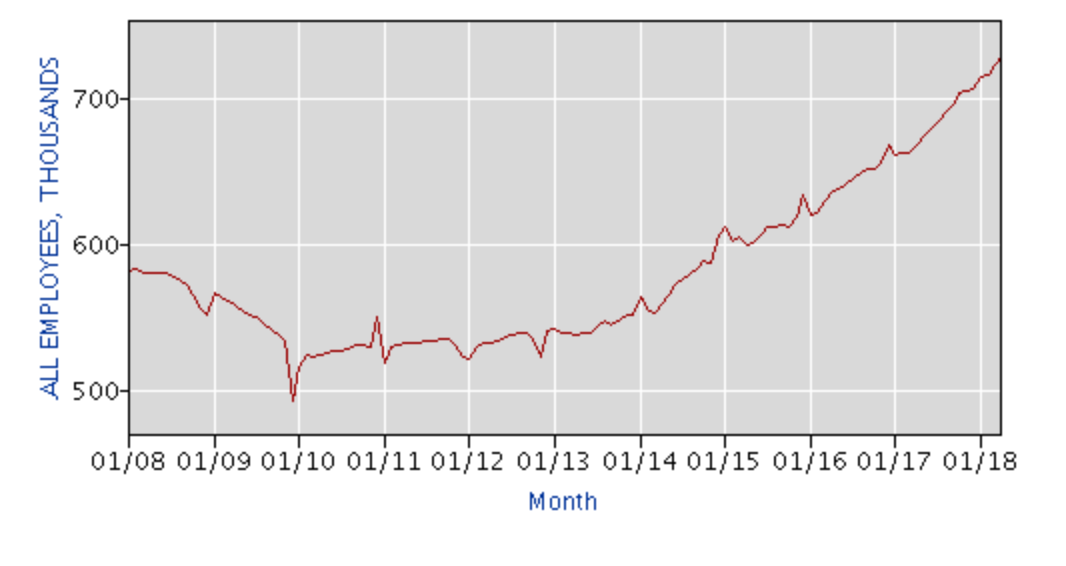
\includegraphics[width=\textwidth]{Figures/sudalgaa/employees.png}
	\caption{Хүргэлтийн үйлчилгээ үзүүлдэг байгууллагуудын ажилчдын тоон өсөлт}
	\label{fig:employee}
\end{figure}
Зураг~\ref{fig:earnings}--т АНУ-д үйл ажиллагаа явуулдаг хүргэлтийн байгууллагуудын ажилчдын цагийн цалингийн өөрчлөлтийг харуулав.
\begin{figure}[H]
	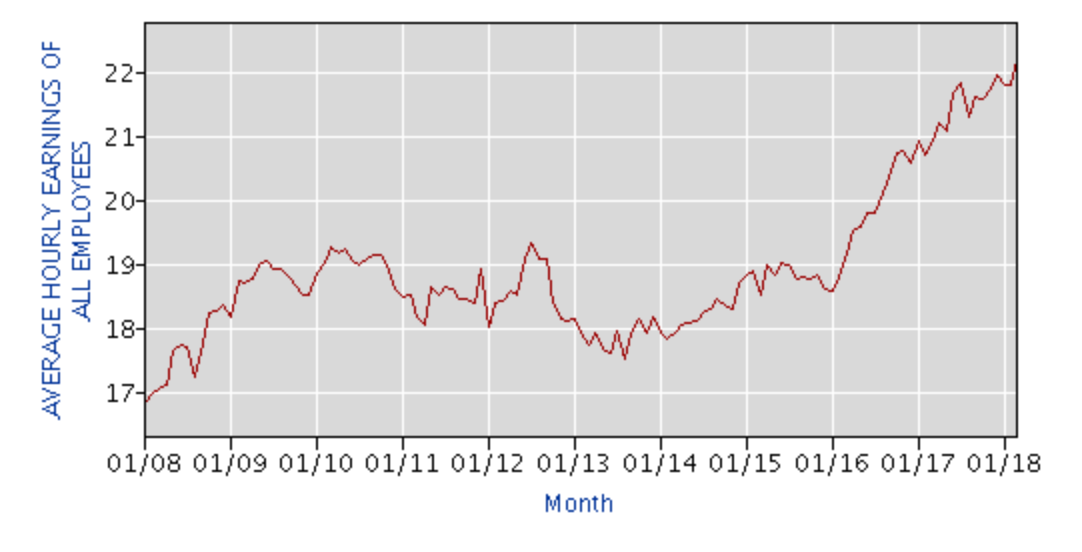
\includegraphics[width=\textwidth]{Figures/sudalgaa/earnings.png}
	\caption{Хүргэлтийн үйлчилгээ үзүүлдэг байгууллагуудын ажилчдын цагийн цалингийн өөрчлөлт\cite{Statics}}
	\label{fig:earnings}
\end{figure}

%---------------------------------------------------------------------------------------
%	SECTION 4
%---------------------------------------------------------------------------------------
\section{Хөгжүүлэлтэд ашиглах технологи, хэрэгслүүд}

\subsection{Риакт (React)-ын тухай}
Риакт (заримдаа React.js эсвэл ReactJS) нь хэрэглэгчийн интерфэйс бүтээхэд зориулсан ЖаваСкрифт сан юм.

Риактыг SPA болон мобайл аппликэйшн хийхэд ашиглаж болдог. Риактын гол баримтлал нь хурд, энгийн байдал болон өргөтгөх боломж юм. Риактыг өөр бусад сангуудтай өргөнөөр ашигладаг бөгөөд тэдгээрийн нэг нь Рэдүкс юм.

SPA (Single Page Application) нь энгийнээр вэб аппликешныг browser дотор ашиглах явцад хуудас дахин дууддагүй аппликешн юм. Таны өдөр бүр л хэрэглэдэг Gmail, Google Maps, Facebook г.м вэб аппликешнууд. SPA нь маш сайн UX -тэй ашиглахад таатай experience үзүүлэх, хуудас дахин дуудахгүй, контент хүлээх шаардлагагүй, доторх контентоо дээд түвшиний javascript фрэймворкууд (Angular, Ember, React)-ын тусламжтай дуудаж харуулдаг.

\subsubsection{Түүх}
Риактыг Фэйсбүүкийн програм хангамжийн инженер Жордан Валкэ нь анх бүтээсэн. Анх тэрээр PHP-д зориулсан HTML бүрэлдэхүүний фрэймворк гаргаж байсан. Үүнийг 2011 онд Фэйсбүүкийн мэдээний фийд дээр ашиглаж эхлэсэн бөгөөд хожим 2012 оноос Инстаграммд хэрэглэх болсон. Риактыг 2013 оны 5-р сард болсон JSConf арга хэмжээнд нээлттэй эх (opensource) болгосон.

\subsubsection{Ялгарах онцлог}
\begin{itemize}[label={--}]
    \item 1 чигийн өгөгдлийн холбоо (One-way data binding).
    \item Нөхцөлт бүрэлдэхүүнүүд.
    \item Хийсвэр DOM.
    \item Амьдралын цикл.
    \item JSX.
    \item HTML-ээс ангид архитектур.
\end{itemize}

\begin{figure}[H]
	\centering
	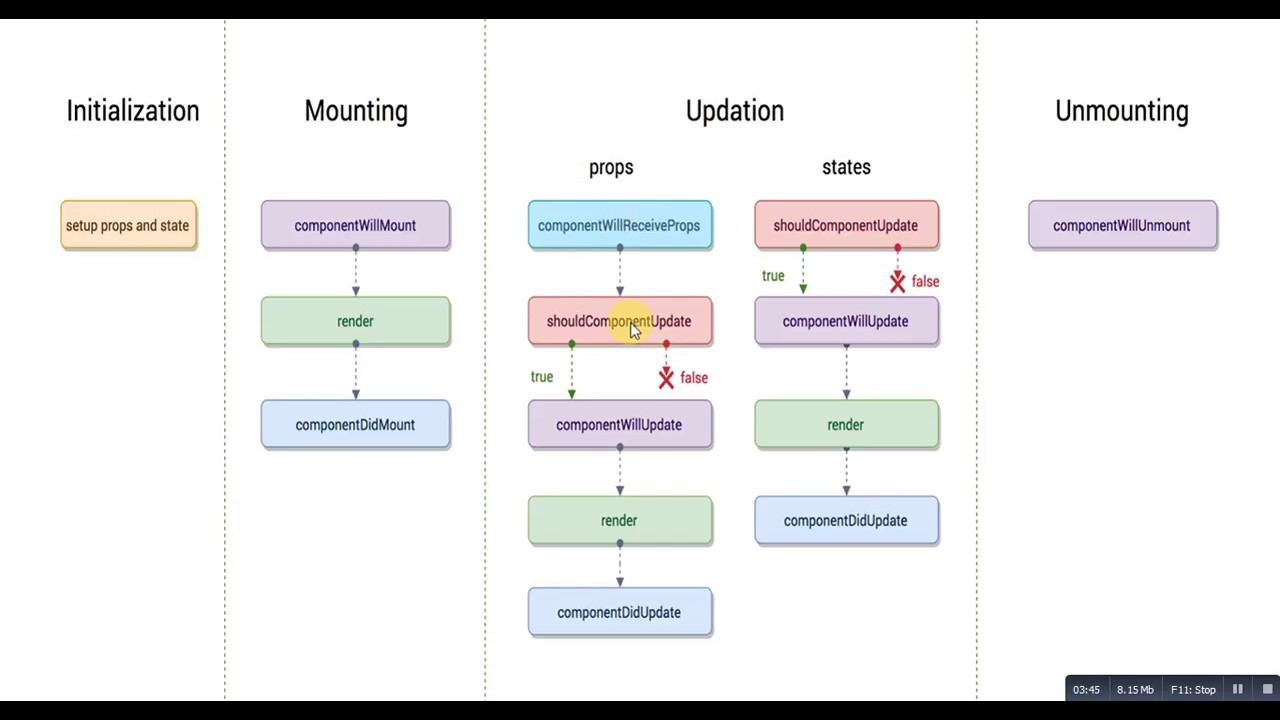
\includegraphics[width=\textwidth]{Figures/sudalgaa/react-lifecycle.jpg}
	\caption{Риакт амьдралын цикл}
	\label{figure:react-lifecycle}
\end{figure}

%----------------------------------------------------------------------
\subsection{Рэдүкс (Redux)-ын тухай}
Рэдүкс нь Жаваскрипт аппуудад зориулсан урдчилан таамаглах боломжтой нөхцөл агуулагч юм.

Рэдүкс нь апп-ны нөхцлүүдийг удирдахад илүү амар болгож өгнө. Өөрөөр хэлбэл хэрэглэгчийн үйлдэлд хэрхэн хариу өгч ямар өгөгдөл харуулахыг удирддаг.

\begin{figure}[H]
	\centering
	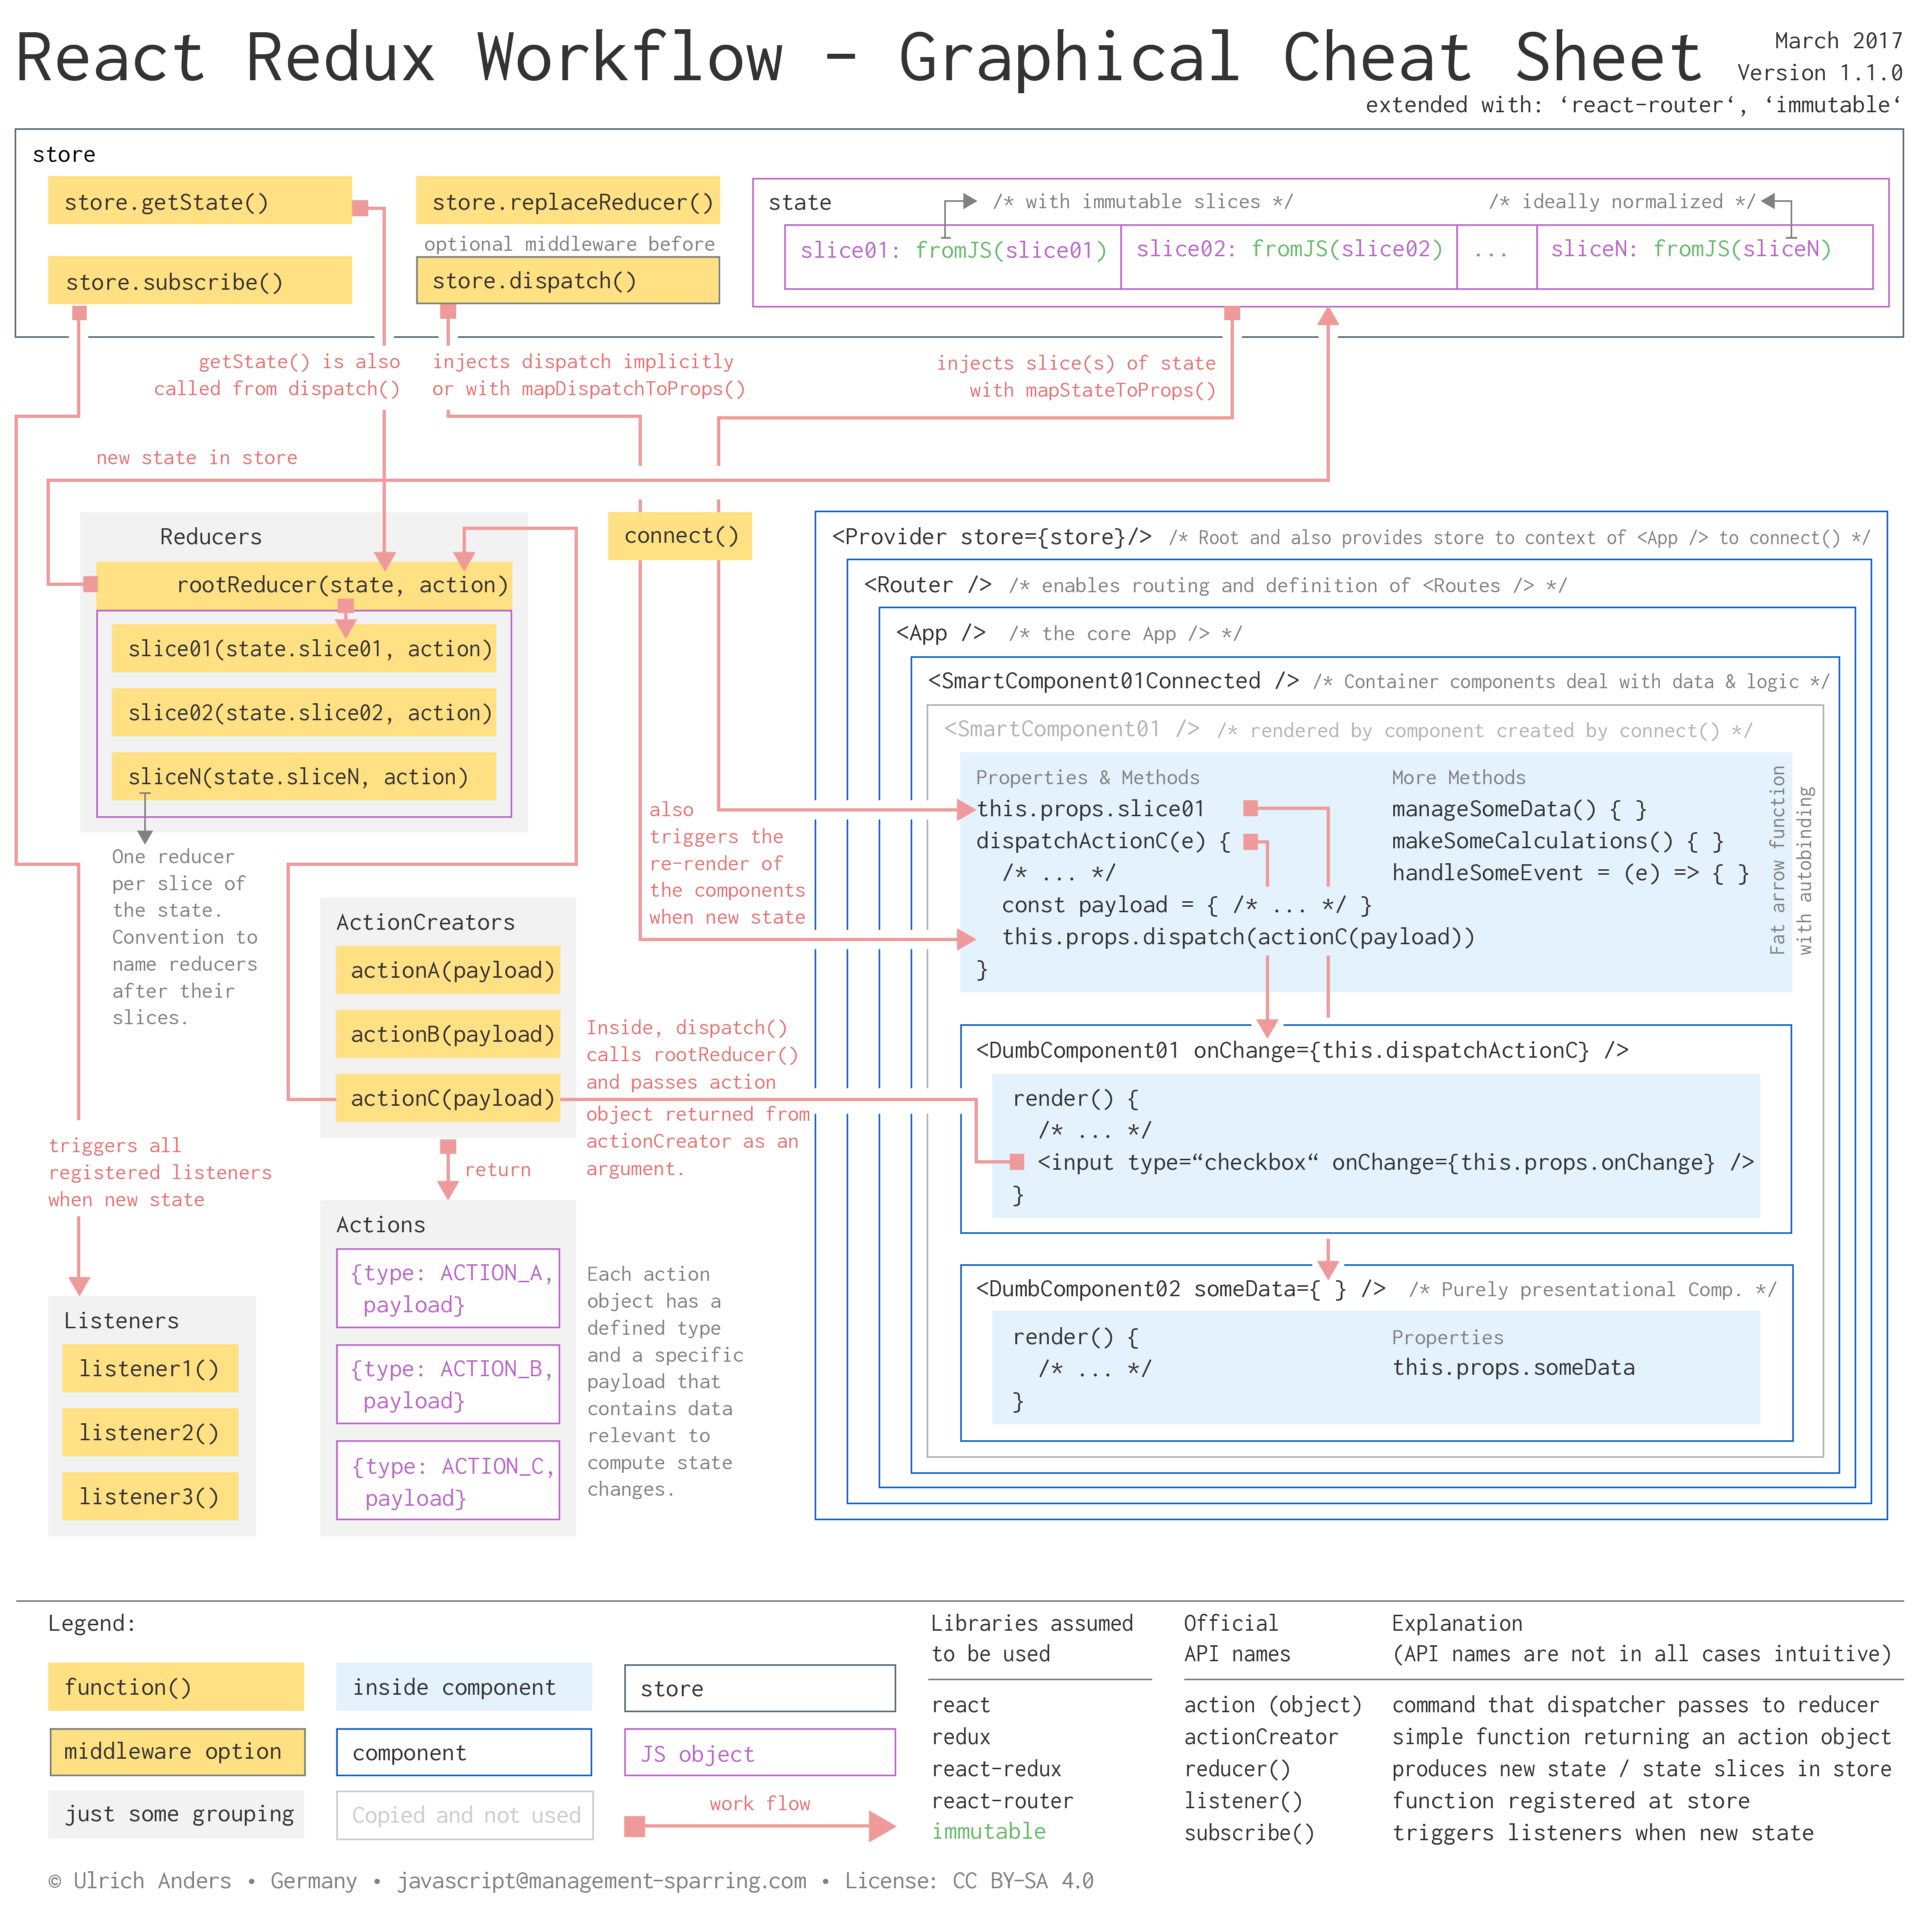
\includegraphics[width=\textwidth]{Figures/sudalgaa/redux-workflow.png}
	\caption{Рэдүкс ажиллах дараалал}
	\label{figure:redux-workflow}
\end{figure}

%----------------------------------------------------------------------
\subsection{Риакт Натив (React Native)-ын тухай}
Риакт Натив нь Жаваскрипт ашиглан мобайл апп хөгжүүлэх боломжийг олгодог. Риакттай яг адил загвар ашигладаг. Objective-C, Java, эсвэл Swift дээр бичсэн бүрэлдэхүүнүүдийг өөгүй нэгтгэнэ. Натийв код ашиглах хэрэг гарсан үед зарим талыг энгийнээр засаж болно. Апп-ны зарим хэсгийг Риакт натив ашиглан зарим хэсгийг Натийв код бичих боломжтой.

% ---------------------------------------------------------------------
\subsection{Экспо (Expo)-ын тухай}
Экспо апп нь Риакт Натийв апп бөгөөд дотроо Экспо SDK агуулна.Уг SDK нь native-and-JS сан бөгөөд төхөөрөмж (Камер, дугаарууд, өгөгдлийн хадгалалт, болон бусад техник хангамж) рүү хандах боломжийг олгодог. Энэ нь заавал натийв код бичихгүйгээр асуудлуудыг шийдэх боломжийг олгоно мөн төслийг зөвхөн Жаваскрипт ашиглан авсаархан байхад тусална. Экспо нь мөн хэрэглэгчийн түгээмэл боловч Риакт Натив үндсэн элементүүдэд байхгүй бүрэлдэхүүн хэсгүүдээр хангадаг. Жишээ нь: icon гэх мэт...

% ---------------------------------------------------------------------
\subsection{Фаирбейс платформ}
Гүүглэ компанийн Файрбейс (Firebase) нь гар утасны аппликейшн хөгжүүлэхэд шаардлагатай бүхий л үйлчилгээг нэг дор хослуулсан маш хүчирхэг платформ юм. 
\begin{figure}[H]
	\centering
	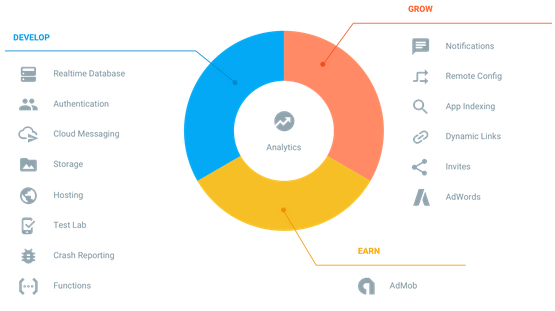
\includegraphics[width=\textwidth]{Figures/sudalgaa/firebase.png}
	\caption{Фаирбейс платформ}
	\label{figure:social}
\end{figure}

\subsubsection{Бодит хугацаатай өгөгдлийн сан}
Фаирбейс-ийн бодит хугацаатай өгөгдлийн сан (Real-time database) нь үүлэнд суурилдаг бөгөөд өгөгдлөө жей-сон форматаар хадгалаж синхроноор өгөгдлийн шинэчлэлтүүдийг системд холбогдсон бүхий л хэрэглэгчдэд хэдхэн миллисекундын дотор автоматаар хийдэг. 

\subsubsection{Хэрэглэгчийн найдвартай байдал}
Ихэнхи аппликейшны нэн тэргүүний хэрэгцээ бол хэрэглэгчдийн мэдээллийг аюулгүй , найдвартайгаар хадгалах юм. Фаирбейс-ийн хэрэглэгчийн найдвартай байдал буюу англиар Authentication нь энэхүү асуудлыг бүрэн цогцоор нь шийдвэрлэж өгсөн байдаг.

\subsubsection{Хадгалалт}
Хэрэглэгчидтэй холбоотой бүхий л төрлийн зураг, видео, файл зэргийг Фаирбейс-ийн хадгалалт(firebase storage) - ийн тусламжтайгаар үүлэнд хадгалах боломжтой байдаг. 

\begin{figure}[H]
	\centering
	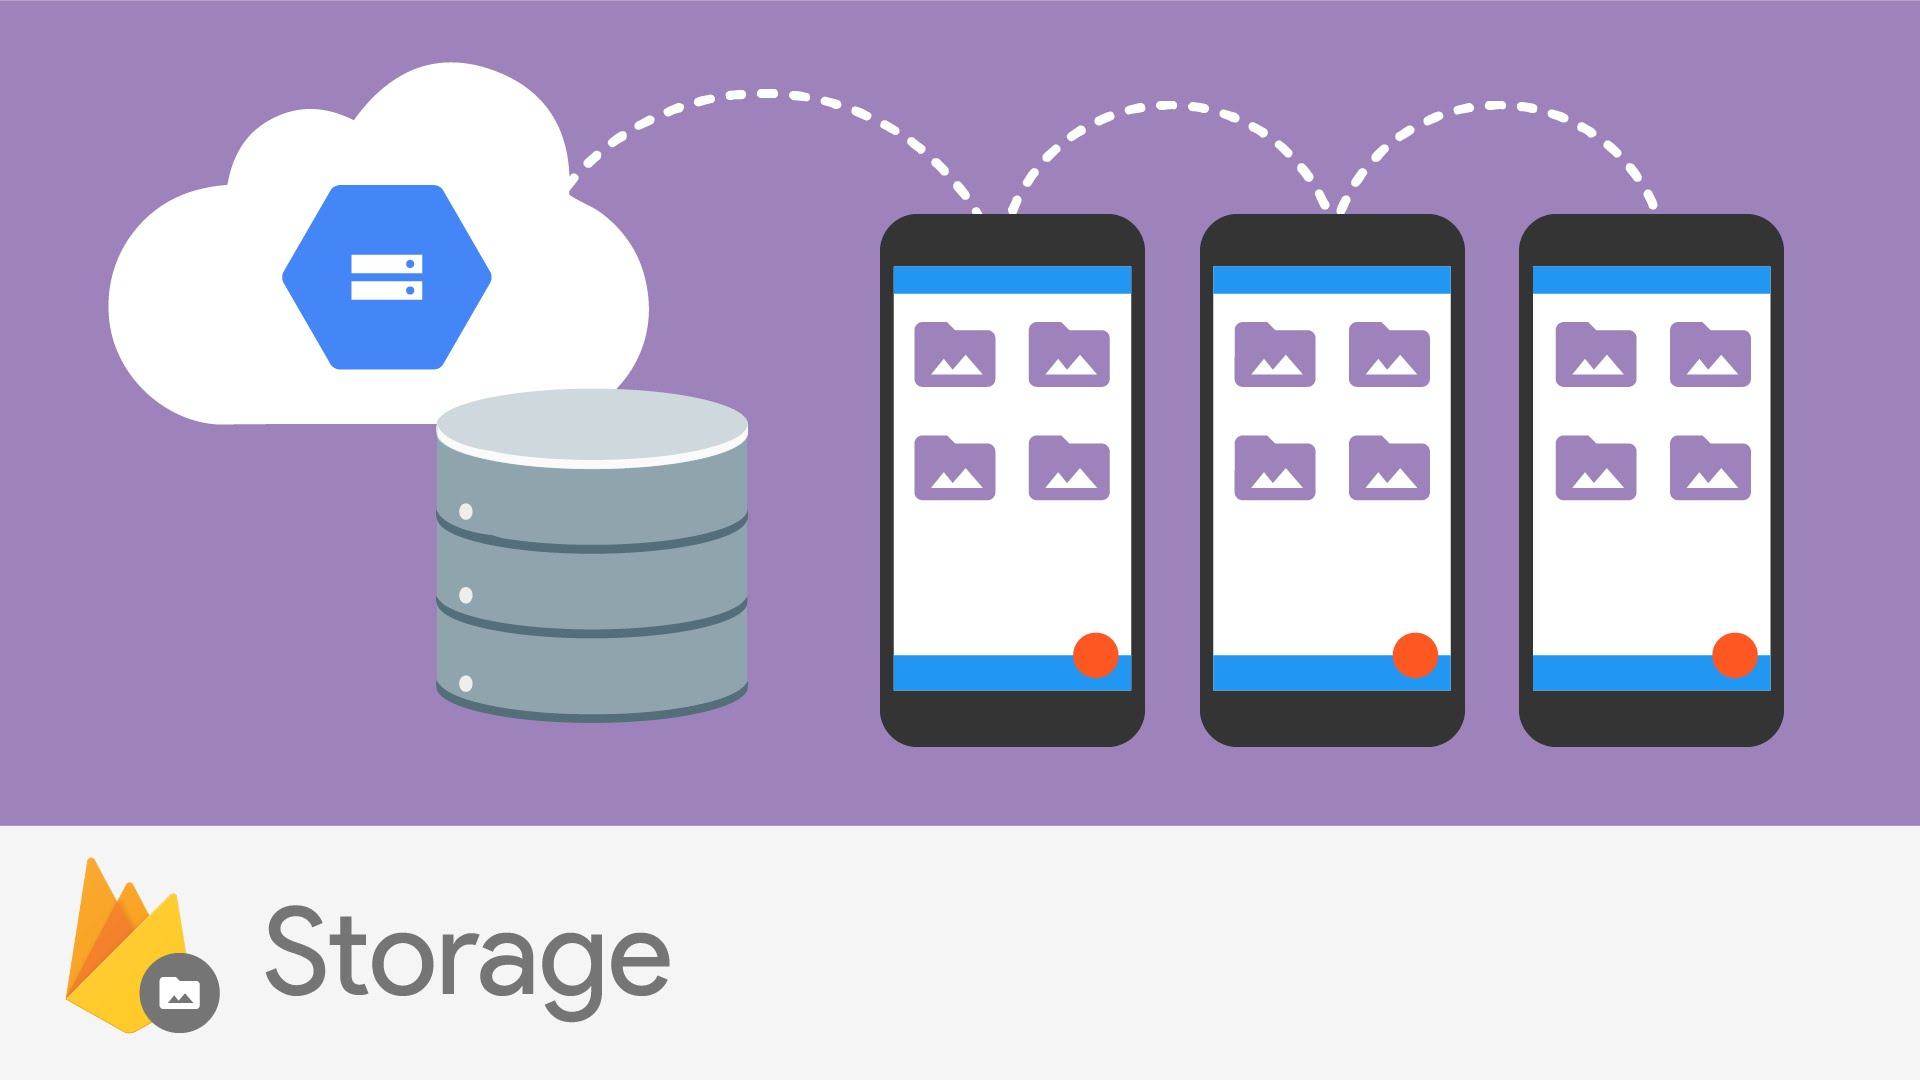
\includegraphics[width=\textwidth]{Figures/sudalgaa/firebaseStorage.jpg}
	\caption{Фаирбейс хадгалалт}
	\label{figure:storage}
\end{figure}

% ---------------------------------------------------------------------
\subsection{Гүүгл Мап (Google Maps)-ын тухай}
Уг Google Maps нь Гүүглэ компаний өөрсдийн газрын зургийг API түлхүүр үгээрээ дамжуулан серверээс өгөгдлөө аван аппликэйшндаа дүрслэх, дурын байршил заах, хэрэглэгчийн байршилын мэдээллийг координатаар тодорхойлох зэрэг үйлдлүүдийг гүйцэтгэж болохоос гадна бусад Google API-уудаар өргөтгөх боломжтой.
\begin{figure}[H]
    \centering
	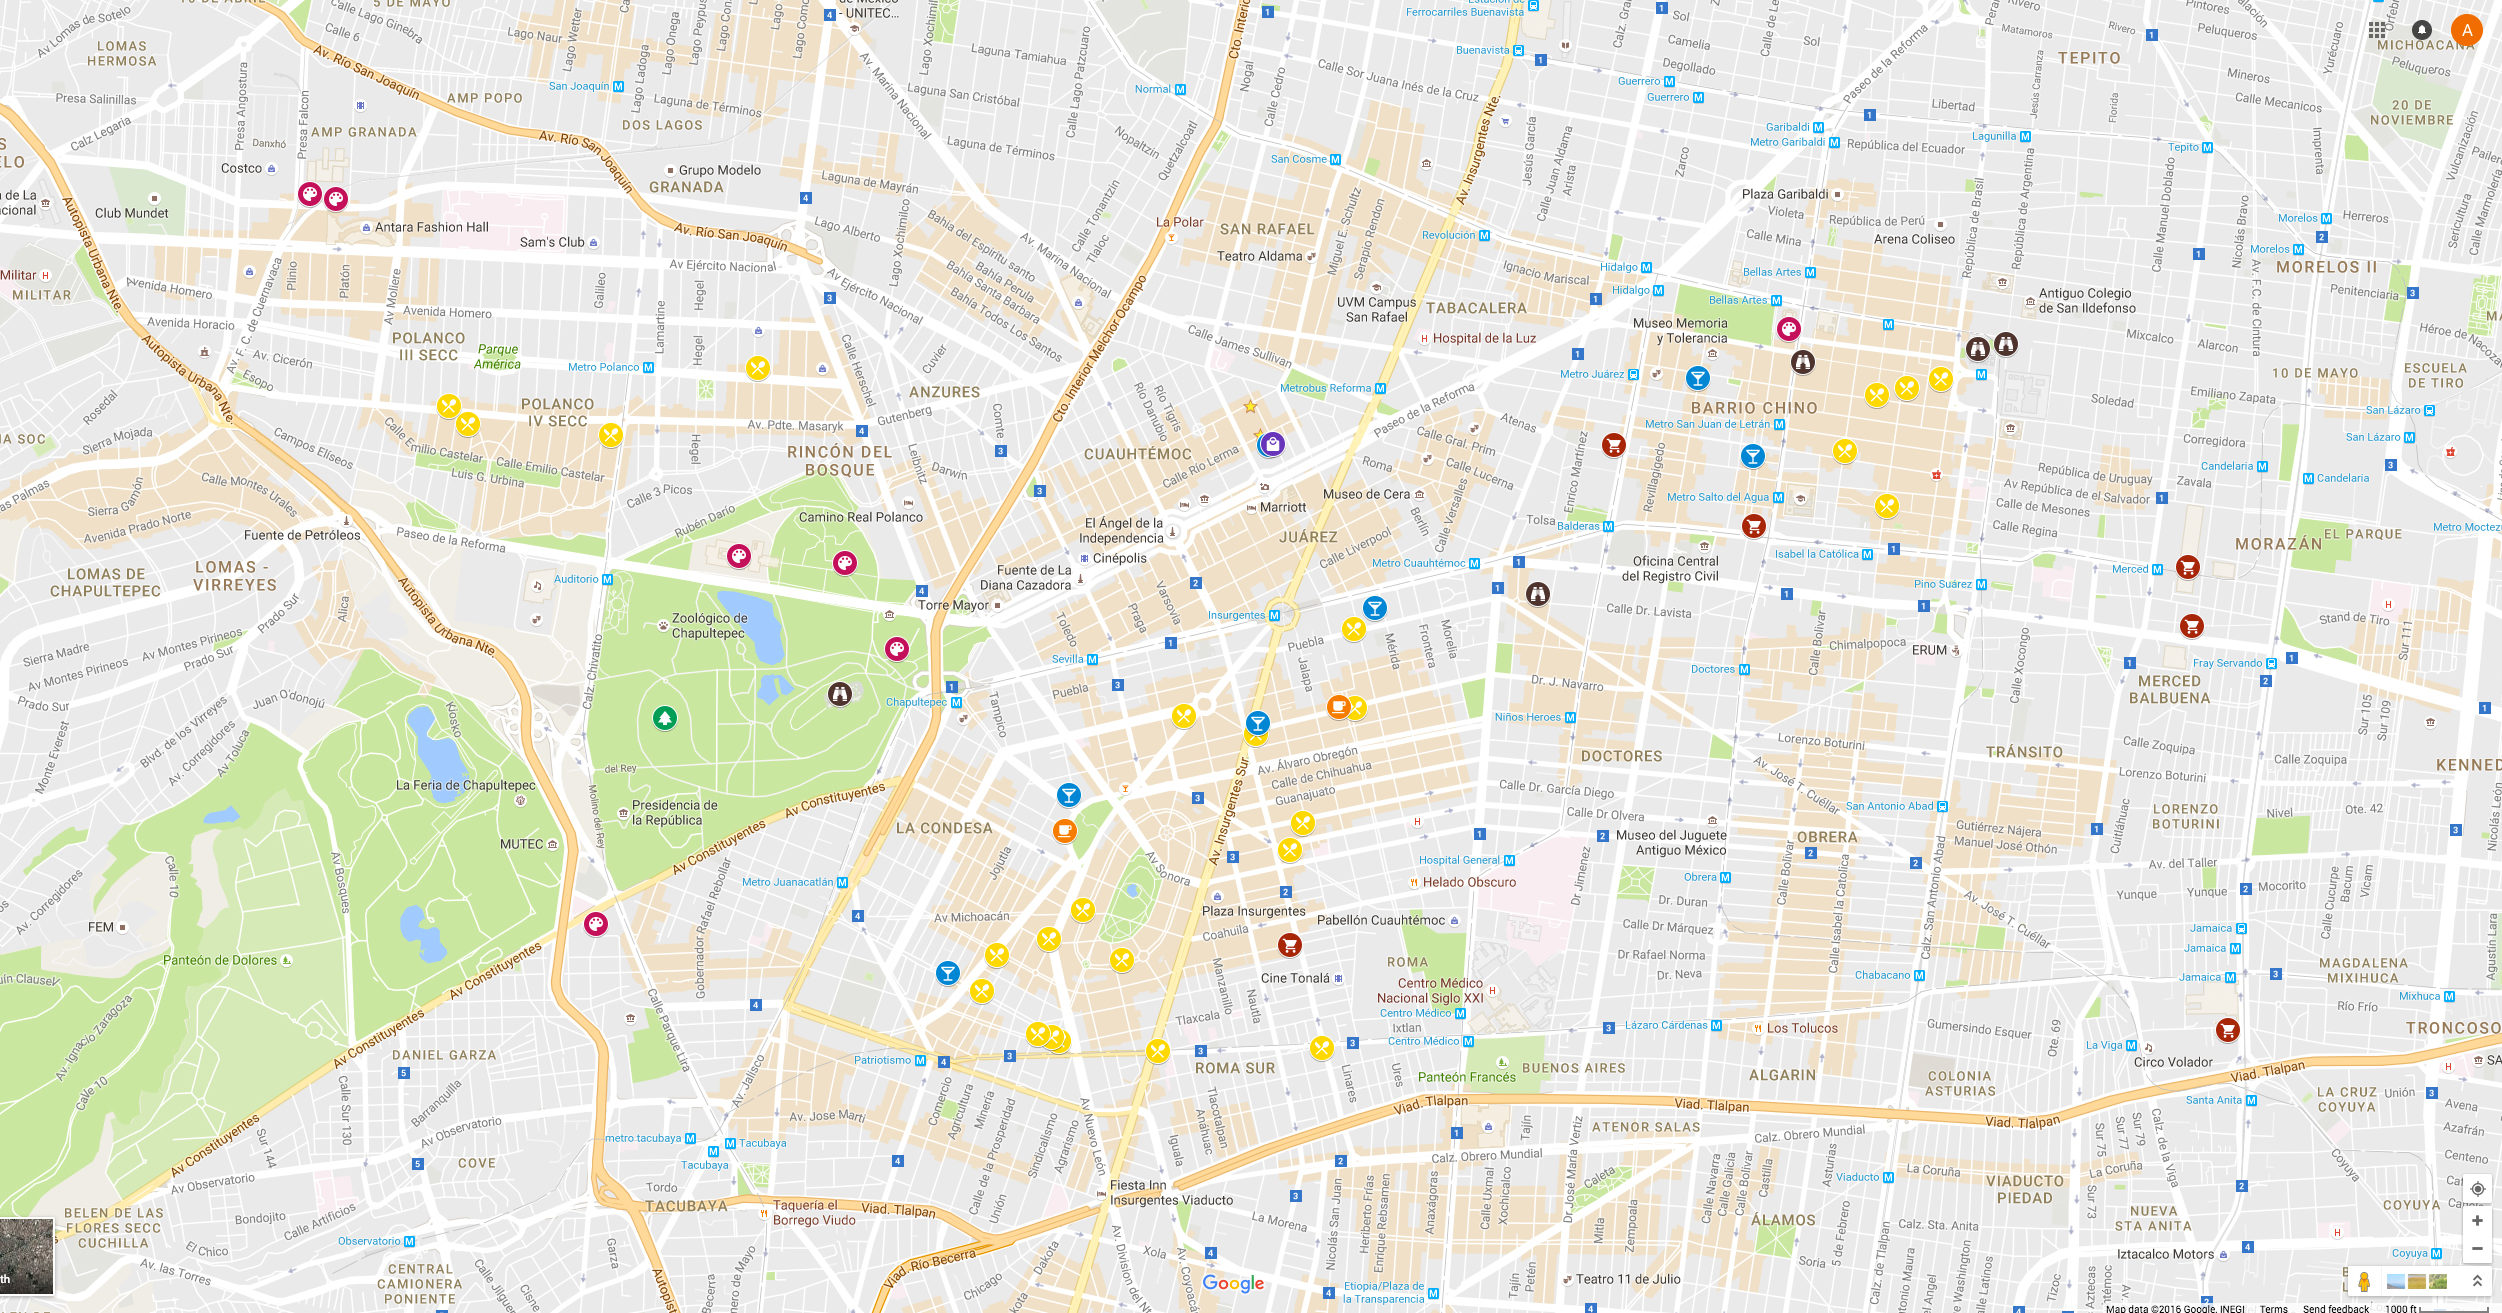
\includegraphics[width=\textwidth]{Figures/sudalgaa/Google-Maps.jpg}
	\caption{Google Maps харагдах байдал.}
	\label{fig:Google-Maps}
\end{figure}
Энэхүү програм хангамж хөгжүүлэх хэрэгслийг ашиглахын тулд Гүүглийн хөгжүүлэгчдийн сайтад нэвтэрч шинэ прожект үүсгэнэ. Дараа нь ашиглах API-аа сонгож API Key буюу түлхүүр үг үүсгэн хадгална.

%---------------------------------------------------------------------------------------
%	SECTION 5
%---------------------------------------------------------------------------------------
\section{Хөгжүүлэлтэнд ашиглах алгоритм}

\subsection{Хамгийн богино зам олох.}
Дээр дурдсан Google Direction API нь тодорхой хоёр байршил хоорондын хамгийн богино тодорхойлж өгдөг API юм.
Уг API-ийн ашиглаж байгаа хамгийн богино зам олох алгоритмууд нь олон тооны бөгөөд дэлхий нийтээр Дейкстра алгоритмыг ашигласан байх магадлал маш өндөр гэж үзэж байгаа.
Учир нь Дэйкстра алгоритм нь хамгийн сүүлийн үеийн хоёр байршил хоорондын хамгийн бага өртөгтэй замыг хайж олдог алгоритм юм.  

%---------------------------------------------------------------------------------------
%	SECTION 6
%---------------------------------------------------------------------------------------
\section{Бүлгийн дүгнэлт}

Энэ бүлгийн хүрээнд уг системийн судалгааны бичиг баримтыг хийж гүйцэтгэсэн ба дараах зүйлсийг тодорхойлов:
\begin{itemize}[label={--}]
    \renewcommand\labelitemi{--}
    \item Системийн тухай танилцуулгыг тодорхойлсон,
    \item Ижил төстэй системийн судалгааг хийсэн,
    \item Тоон судалгааг хийсэн,
    \item Хөгжүүлэлтэд ашиглагдах алгоритмыг тодорхойлсон,
    \item Хөгжүүлэлтэд ашиглах технологи, хэрэгслүүдийг тодорхойлсон болно.
\end{itemize}

%-------------------------------------------------------------------------------